\pdfinfoomitdate=1
\pdftrailerid{}
\pdfsuppressptexinfo=15
\documentclass[11pt]{article}
\usepackage[T1]{fontenc}
\usepackage{lmodern}
\usepackage[margin=1.05in]{geometry}
\usepackage{amsmath,amssymb,amsthm,mathtools}
\usepackage{microtype}
\usepackage{enumitem}
\usepackage{xcolor}
\usepackage{tikz}
\usetikzlibrary{arrows.meta,positioning,calc,fit}
\usepackage[colorlinks=true,linkcolor=blue!45!black,citecolor=green!35!black,urlcolor=blue!55!black]{hyperref}
\hypersetup{pdftitle={A nine-dimensional counterexample to Borsuk's covering assertion},pdfauthor={OpenAI}}
\usepackage[nameinlink,noabbrev]{cleveref}
\newtheorem{theorem}{Theorem}[section]
\newtheorem{proposition}[theorem]{Proposition}
\newtheorem{lemma}[theorem]{Lemma}
\newtheorem{corollary}[theorem]{Corollary}
\theoremstyle{definition}
\newtheorem{definition}[theorem]{Definition}
\theoremstyle{remark}
\newtheorem{remark}[theorem]{Remark}
\numberwithin{equation}{section}
\DeclareMathOperator{\tr}{tr}
\DeclareMathOperator{\rank}{rank}
\DeclareMathOperator{\Sym}{Sym}
\DeclareMathOperator{\supp}{supp}
\setlist{nosep}
\setlength{\emergencystretch}{1em}

\title{A nine-dimensional counterexample to Borsuk's covering assertion}
\author{OpenAI}
\date{September 23, 2026}
\begin{document}
\maketitle
\begin{abstract}
The compact set of rank-one orthogonal projectors on $\mathbb R^4$,
with the Frobenius metric, cannot be covered by ten sets of strictly
smaller diameter. It therefore gives a counterexample to Borsuk's
conjecture in dimension nine.
\end{abstract}
\setcounter{tocdepth}{1}
\tableofcontents
\clearpage
\section{Introduction}
\label{sec:introduction}

Borsuk's partition problem asks whether every bounded set of positive
diameter in $\mathbb R^d$ can be covered by $d+1$ subsets of strictly
smaller diameter. For a bounded set $Y$ of positive diameter, write $b(Y)$ for the least
number of such subsets needed to cover $Y$. Covers and partitions give
the same number: overlaps may be removed without increasing diameters.
We prove that $b(Y)>10$ for a compact set in $\mathbb R^9$.

Let $\operatorname{Sym}_4(\mathbb R)$ be the space of real symmetric
$4\times4$ matrices, with Frobenius norm
$\|A\|_F^2=\operatorname{tr}(A^2)$. Its trace-one affine hyperplane is
a nine-dimensional Euclidean space. For a unit vector $u\in\mathbb R^4$,
the matrix $uu^{\mathsf T}$ is the orthogonal projector onto the line
spanned by $u$.

\begin{theorem}\label{thm:main}
The compact set
\[
 X=\{uu^{\mathsf T}:u\in\mathbb R^4,\ \|u\|=1\}
 \subset\{A\in\operatorname{Sym}_4(\mathbb R):\operatorname{tr}A=1\},
\]
with the Frobenius metric, has diameter $\sqrt2$ and cannot be covered
by ten subsets of diameter strictly less than $\sqrt2$.
\end{theorem}

Thus Borsuk's assertion fails in dimension nine. The theorem does not
determine the smallest dimension in which it fails
or the exact value of $b(X)$. Its witness is the full compact projector
image of real projective three-space. Corollary~\ref{cor:higher-dimensions}
extends the construction to compact counterexamples in every dimension
$d\geq9$.

\subsection*{History and the method}
Borsuk posed the partition question in 1933 \cite{Borsuk1933}.
Kahn and Kalai disproved it in high dimensions \cite{KahnKalai1993},
using a forbidden-intersection theorem of Frankl and Wilson
\cite{FranklWilson1981} to force many smaller-diameter parts.
Early reductions in counterexample dimension include $946$
by Nilli \cite{Nilli1994}, the announced bound $903$ of Grey and
Weissbach \cite{GreyWeissbach1997}, $561$ by Raigorodskii
\cite{Raigorodskii1997}, and $560$ by Weissbach \cite{Weissbach2000}.

Spherical codes led to a further series of reductions. Hinrichs obtained
dimension $323$ using vectors of the Leech lattice
\cite{Hinrichs2002}. Pikhurko reduced the bound to $321$ and credited
an independent discovery by Hinrichs and Richter \cite{Pikhurko2002};
Hinrichs and Richter published their bound $298$ in 2003
\cite{HinrichsRichter2003}.

A different series of advances used strongly regular graphs.
Bondarenko constructed a two-distance counterexample in dimension $65$
\cite{Bondarenko2014}; Jenrich and Brouwer obtained dimension $64$
\cite{JenrichBrouwer2014}. Grinsztajn's public proof note gives a
finite counterexample in dimension $63$ \cite{Grinsztajn2026}.
Theorem~\ref{thm:main} improves this dimension bound using the full
compact image of projective space rather than a finite configuration.

The projector embedding itself is classical. Kalai describes the map
$x\mapsto x\otimes x$ and the full rank-one positive semidefinite
configuration in his account of the Kahn--Kalai construction
\cite[Section~2.3]{Kalai2015}. Conway, Hardin, and Sloane use the
same projection-matrix model for Grassmannian packing and its Euclidean
metric \cite[Section~5, Theorem~2]{ConwayHardinSloane1996}.
Our contribution is the covering obstruction for the projector set
associated with $\mathbb R^4$.

The relevant topological antecedents include Walkup's eleven-vertex
minimum for triangulations of $\mathbb{RP}^3$
\cite[Theorem~3]{Walkup1970} and the projective-space vertex bounds
of Arnoux and Marin \cite{ArnouxMarin1991}. These results cannot be
applied directly to the complex here: its faces are positive coordinate
supports of a map, not simplices in a triangulation of projective space.
The central difficulty is to derive enough of its face structure from
the map itself. We do this through an odd map on symmetric matrices,
mod-two degree, and local preimage counts, and then give the finite
combinatorial obstruction in full.

\subsection*{Proof overview}
Two projectors in $X$ are at diameter distance precisely when their
underlying lines are orthogonal. A hypothetical cover by ten sets of
strictly smaller diameter can be enlarged to an open cover. A smooth
partition of unity then gives nonnegative functions $f_1,\ldots,f_{10}$
on $\mathbb{RP}^3$, with sum one, such that orthogonal lines have disjoint
sets of positive coordinates. Section~\ref{sec:geometry} proves this
reduction for arbitrary covering sets.

We record these sets of positive coordinates in a finite simplicial
complex: a set of labels is a face if all its coordinates are positive
at some line. To constrain this complex, Section~\ref{sec:extension}
extends the map $f$ to positive semidefinite matrices by integration,
then subtracts its values on the positive and negative parts of a
symmetric matrix. For the resulting odd map, the sum of the absolute output coordinates
equals the sum of the absolute eigenvalues of the input matrix.
Normalizing these two sums gives an odd map between spheres. In Section~\ref{sec:topology}, its mod-two
degree forces every maximal support to have four labels and the sum of
these tetrahedral faces to be a cycle.

The main topological step is the equality argument in
Section~\ref{sec:topology}. At the threshold of $k(k+1)/2$ labels on
$\mathbb{RP}^{k-1}$, a maximal support with fewer than $k$ labels
would give a positive-dimensional regular level set inside one affine
projective chart. Applying the matrix extension on the orthogonal
complement of each line gives a map on a sphere bundle over this level
set. The odd degree of the original extension forces an odd preimage
count for this map, whereas the chart trivialization makes the same
count even through the induced map on the projective bundle. Once every maximal support has
$k$ labels, the remaining odd local counts determine the coefficients
of the facet cycle.

The last stage converts this topological information into a finite
obstruction. The same degree argument in $\mathbb R^3$ produces a rigid triangle system on six
labels, described in Section~\ref{sec:six-labels}. Each tetrahedral face
of the ten-label complex forces such a system on its six-label
complement. Once these systems have been derived,
Section~\ref{sec:ten-labels} follows them across adjacent tetrahedra by
purely combinatorial arguments. Their compatibility restricts the cycles
around edges and organizes a subset of the labels into small blocks.
The blocks and the remaining labels give the final contradiction.
Section~\ref{sec:conclusion} returns to the diameter cover.

\section{From diameter covers to projective maps}
\label{sec:geometry}

The geometric part of the proof converts a smaller-diameter cover into a
smooth map whose positive coordinates separate orthogonal lines.  We first
make this conversion explicit, so that the remaining obstruction can be
formulated entirely on projective space.

The projection-matrix metric is the rank-one case of the standard
Euclidean embedding of real Grassmannians
\cite[Section~5, Theorem~2]{ConwayHardinSloane1996}. Their chordal
distance is $1/\sqrt2$ times the Frobenius distance used here. We give
the short computation to fix the normalization throughout the proof.

Let $V=\mathbb R^k$ have its usual inner product, with $k\geq2$, and let
$\mathbb P(V)$ denote its space of one-dimensional linear subspaces.
For a line $x=[u]$, represented by a unit vector $u$, write $P_x=uu^{\mathsf T}$
for the orthogonal projector onto $x$.  Let $\operatorname{Sym}(V)$ be the
space of real symmetric operators, equipped with the Frobenius inner product
$\langle A,B\rangle_F=\operatorname{tr}(AB)$, and put
\[
 N_k=\dim\operatorname{Sym}(V)=\frac{k(k+1)}2,
 \qquad X_k=\{P_x:x\in\mathbb P(V)\}.
\]

\begin{lemma}[Projector geometry]
\label{lem:projector-geometry}
The map $x\mapsto P_x$ identifies $\mathbb P(V)$ homeomorphically with the
compact set $X_k$ in the trace-one affine subspace of
$\operatorname{Sym}(V)$.  This affine subspace is Euclidean of dimension
$N_k-1$.  If $u,v$ are unit representatives of $x,y$, then
\begin{equation}
 \|P_x-P_y\|_F^2=2-2\langle u,v\rangle^2.
 \label{eq:projector-distance}
\end{equation}
Consequently $\operatorname{diam}(X_k)=\sqrt2$, and two projectors are at
this distance exactly when their lines are orthogonal.
\end{lemma}

\begin{proof}
The formula $uu^{\mathsf T}$ is unchanged when $u$ is replaced by $-u$,
so it gives a continuous map on projective space.  Its range as an operator
is exactly $x$, which proves injectivity.  A continuous injection from the
compact space $\mathbb P(V)$ into a Hausdorff space is a homeomorphism onto
its image.  Every $P_x$ has trace one, and the trace-one hyperplane has
codimension one in $\operatorname{Sym}(V)$.  Finally,
$\operatorname{tr}(P_x^2)=\operatorname{tr}(P_y^2)=1$ and
$\operatorname{tr}(P_xP_y)=\langle u,v\rangle^2$, proving
\eqref{eq:projector-distance}.  Orthogonal lines exist because $k\geq2$.
\end{proof}

\begin{remark}[Euclidean coordinates]
An explicit isometry from the trace-one symmetric $4\times4$
matrices to $\mathbb R^9$ is
\begin{equation}
\begin{split}
 A\longmapsto\bigg(&\frac{a_{11}-a_{22}}{\sqrt2},\;
 \frac{a_{11}+a_{22}-2a_{33}}{\sqrt6},\;
 \frac{a_{11}+a_{22}+a_{33}-3a_{44}}{\sqrt{12}},\\
 &\sqrt2a_{12},\sqrt2a_{13},\sqrt2a_{14},
   \sqrt2a_{23},\sqrt2a_{24},\sqrt2a_{34}\bigg).
\end{split}
\label{eq:euclidean-coordinates}
\end{equation}
The first three coordinates use an orthonormal basis of the trace-zero
diagonal matrices.  The factors $\sqrt2$ in the remaining six coordinates
account for the two equal off-diagonal entries in the Frobenius norm.
Thus the nine-dimensional witness will be $X_4$ with exactly its stated
metric.
\end{remark}

Write $[m]=\{1,\ldots,m\}$ and
$\Delta^{m-1}=\{(t_1,\ldots,t_m):t_i\ge0,\ \sum_i t_i=1\}$.

\begin{definition}
\label{def:admissible}
A smooth map $f=(f_1,\ldots,f_m):\mathbb P(V)\to\mathbb R^m$ is
\emph{admissible} if each $f_i$ is nonnegative, $\sum_i f_i=1$, and,
writing $S(x)=\{i:f_i(x)>0\}$,
\begin{equation}
 x\perp y\quad\Longrightarrow\quad S(x)\cap S(y)=\varnothing.
 \label{eq:admissibility}
\end{equation}
Here smoothness means smoothness of the real coordinate functions on the
usual smooth manifold $\mathbb P(V)$.
\end{definition}

Restricting an admissible map to $\mathbb P(W)$ for a nonzero linear
subspace $W\subseteq V$ preserves admissibility.  Coordinates that vanish
identically on this subspace may be omitted.

\begin{lemma}[The strict-gap reduction]
\label{lem:cover-to-map}
If $X_k$ is covered by at most $m$ subsets, each of diameter strictly less
than $\sqrt2$, then there is an admissible map
$f:\mathbb P(V)\to\mathbb R^m$.
\end{lemma}

\begin{proof}
Pad the cover by empty sets to write it as $A_1,\ldots,A_m$.
For every nonempty $A_i$, set $d_i=\operatorname{diam}(A_i)$ and
$\varepsilon_i=(\sqrt2-d_i)/4>0$, and define the relatively open set
\[
 U_i=\{P\in X_k:\operatorname{dist}_F(P,A_i)<\varepsilon_i\}.
\]
Set $U_i=\varnothing$ if $A_i=\varnothing$.  The sets $U_i$ cover $X_k$.
For any $P,Q\in U_i$, points of $A_i$ within $\varepsilon_i$ of $P,Q$
and the triangle inequality give
\[
 \|P-Q\|_F<d_i+2\varepsilon_i
 =\frac{d_i+\sqrt2}{2}<\sqrt2.
\]
In particular $\operatorname{diam}(U_i)\leq(d_i+\sqrt2)/2<\sqrt2$.

Pull these sets back to a finite open cover $V_i$ of $\mathbb P(V)$.
A smooth partition of unity subordinate to this cover
\cite[Theorem~2.23]{Lee2013} gives smooth
nonnegative functions $f_i$, with sum one and $f_i(x)>0$ only if
$x\in V_i$.  Empty sets receive the zero function.  If $i$ belonged to
both $S(x)$ and $S(y)$ for orthogonal lines $x,y$, then $P_x,P_y\in U_i$
would be at distance $\sqrt2$ by Lemma~\ref{lem:projector-geometry},
a contradiction.
\end{proof}

The strict diameter inequalities are what permit the open neighborhoods
and the smooth partition of unity; merely excluding individual orthogonal
pairs from arbitrary color classes does not supply this reduction.

For an admissible map, define its \emph{support complex} $K$ on the label
set $\{1,\ldots,m\}$ by
\[
 I\in K\quad\Longleftrightarrow\quad
 I\subseteq S(x)\ \text{for some }x\in\mathbb P(V).
\]
It is a finite simplicial complex, possibly with unused labels, and $f$
takes values in its geometric realization inside the standard simplex.
No triangulation of $\mathbb P(V)$ is assumed.  The next sections derive
the properties of $K$ that will rule out an admissible map when $k=4$ and
$m=10$.

\section{An extension to symmetric matrices}
\label{sec:extension}

Fix an admissible map $f:\mathbb P(V)\to\mathbb R^m$, where
$\dim V=k$.  We extend $f$ first to positive semidefinite operators and
then to all symmetric operators.  Orthogonal spectral subspaces will give
disjoint sets of labels, producing an odd map between spheres.

Define the continuous degree-two homogeneous function
$H:V\to\mathbb R^m$ by
\[
 H(v)=\begin{cases}\|v\|^2f([v]),&v\ne0,\\0,&v=0.\end{cases}
\]
Continuity at zero follows from $\|H(v)\|_1=\|v\|^2$.
For a positive semidefinite operator $Q$, let
\begin{equation}
 E_V(Q)=k\int_{\mathbb S(V)}H(Q^{1/2}u)\,d\mu_V(u),
 \label{eq:extension}
\end{equation}
where $\mu_V$ is rotation-invariant probability measure on the unit sphere.
The positive square root is meant throughout.  We usually write $E$
when the ambient space is clear.

\begin{lemma}[Properties of the positive extension]
\label{lem:positive-extension}
The map $E_V$ is continuous on the full positive semidefinite cone,
including its singular boundary.  For $t\geq0$ it satisfies
\[
 E_V(tQ)=tE_V(Q),\qquad E_V(Q)_i\geq0,\qquad
 \sum_{i=1}^m E_V(Q)_i=\operatorname{tr}Q.
\]
Its positive coordinates are exactly the labels used on the range of $Q$:
\begin{equation}
 \{i:E_V(Q)_i>0\}
 =\bigcup_{x\in\mathbb P(\operatorname{ran}Q)}S(x),
 \label{eq:extension-support}
\end{equation}
where the right side is empty for $Q=0$.  Moreover:
\begin{enumerate}
\item $E_V(P_x)=f(x)$ for every line $x$;
\item if $Q$ is supported on a nonzero subspace $W\subseteq V$, then
$E_V(Q)=E_W(Q|_W)$, where the latter construction uses $f|_{\mathbb P(W)}$
and the factor $\dim W$;
\item this last expression is smooth when $W$ varies smoothly with fixed
dimension and $Q|_W$ varies smoothly through positive definite operators.
\end{enumerate}
\end{lemma}

\begin{proof}
The positive square root depends continuously on a positive semidefinite
matrix.  For example, approximate the square-root function uniformly by
polynomials on a compact interval containing the spectra under
consideration, and apply those polynomials to the matrices.
Thus the integrand in \eqref{eq:extension} is jointly continuous in
$(Q,u)$; integration over the compact sphere proves continuity of $E_V$.
Its homogeneity and nonnegativity follow from the corresponding properties
of $H$.  Since $\sum_i H(v)_i=\|v\|^2$ and
$\int uu^{\mathsf T}\,d\mu_V(u)=k^{-1}I$, we have
\[
 \sum_i E_V(Q)_i=k\int\langle Qu,u\rangle\,d\mu_V(u)
 =\operatorname{tr}Q.
\]

Every nonzero $Q^{1/2}u$ lies in $\operatorname{ran}Q$.
Conversely, every line in that range is spanned by some $Q^{1/2}u$ with
$\|u\|=1$, because $Q^{1/2}$ is invertible on its range.
If $f_i$ is positive on such a line, the $i$th integrand is positive at
that $u$, and hence on a nonempty open set of the sphere.  Such a set has
positive measure.  This proves \eqref{eq:extension-support} in both
directions.  For $Q=P_x$, every nonzero integrand is a scalar multiple
of $f(x)$, and the scalars integrate to $\operatorname{tr}P_x=1$.
Thus $E_V(P_x)=f(x)$.

To prove the subspace identity, write $r=\dim W$ and let $\pi_W$ be
orthogonal projection.  The finite measure on $\mathbb S(W)$ defined by
\[
 B\longmapsto\int_{\mathbb S(V)}
 \|\pi_Wu\|^2\,\mathbf1_{\{\pi_Wu\ne0,\;
                  \pi_Wu/\|\pi_Wu\|\in B\}}\,d\mu_V(u)
\]
is invariant under all orthogonal transformations of $W$.  Its total mass is
$\int\|\pi_Wu\|^2\,d\mu_V(u)=r/k$, so it equals
$(r/k)\mu_W$.  Because $Q$ vanishes on $W^\perp$ and $H$ is homogeneous
of degree two, this gives
\[
 k\int_{\mathbb S(V)}H(Q^{1/2}u)\,d\mu_V(u)
 =r\int_{\mathbb S(W)}H((Q|_W)^{1/2}w)\,d\mu_W(w),
\]
as claimed.

Finally choose, locally in the parameters, a smooth orthonormal frame
$T:\mathbb R^r\to W$.  Write $Q|_W$ in that frame as the positive
definite matrix $C$.  The subspace formula becomes
\[
 E_V(Q)=r\int_{\mathbb S^{r-1}}H(TC^{1/2}w)\,d\mu(w).
\]
The matrix square root is smooth on positive definite matrices, and
$TC^{1/2}w$ never vanishes.  The function $H$ is smooth away from zero.
Differentiating this expression over the compact sphere proves the
asserted local smoothness.
\end{proof}

For a symmetric operator $A$, let $|A|=(A^2)^{1/2}$ and
$A_+=(|A|+A)/2$, $A_-=(|A|-A)/2$.  These are its positive and negative
parts, so $A=A_+-A_-$ and their ranges are orthogonal.  Define
\begin{equation}
 F(A)=E_V(A_+)-E_V(A_-).
 \label{eq:signed-extension}
\end{equation}

\begin{lemma}[The odd sphere map]
\label{lem:signed-extension}
The map $F:\operatorname{Sym}(V)\to\mathbb R^m$ is continuous, odd,
and homogeneous of degree one for nonnegative scalars.  It satisfies
\begin{equation}
 \|F(A)\|_1=\operatorname{tr}|A|,
 \qquad \sum_iF(A)_i=\operatorname{tr}A.
 \label{eq:extension-norms}
\end{equation}
More precisely, its positive and negative label sets are
\begin{equation}
\begin{aligned}
 \{i:F(A)_i>0\}&=\bigcup_{x\in\mathbb P(\operatorname{ran}A_+)}S(x),\\
 \{i:F(A)_i<0\}&=\bigcup_{x\in\mathbb P(\operatorname{ran}A_-)}S(x).
\end{aligned}
 \label{eq:spectral-support}
\end{equation}
If every coordinate of $F(A)$ is nonzero, then $A$ is nonsingular.
If all coordinates of $F(A)$ are strictly negative, then $A$ is negative
definite; the analogous statement holds with both signs reversed.
The map $F$ is smooth on the open set of nonsingular symmetric operators.
In particular, it restricts to a continuous odd map
\begin{equation}
 \{A:\operatorname{tr}|A|=1\}\longrightarrow
 \{y\in\mathbb R^m:\|y\|_1=1\}.
 \label{eq:norm-sphere-map}
\end{equation}
\end{lemma}

\begin{proof}
Continuity and homogeneity follow from Lemma~\ref{lem:positive-extension}
and the continuous formulas for $A_\pm$.  Replacing $A$ by $-A$ exchanges
$A_+$ and $A_-$, so $F$ is odd.  Any line in
$\operatorname{ran}A_+$ is orthogonal to every line in
$\operatorname{ran}A_-$.  Admissibility and
\eqref{eq:extension-support} therefore imply that $E_V(A_+)$ and
$E_V(A_-)$ have disjoint positive coordinates.  There is no cancellation
in their difference.  This proves \eqref{eq:spectral-support} and, by
summing coordinates, \eqref{eq:extension-norms}.

If $\ker A$ contains a line $x$, choose $i\in S(x)$, which is possible
because $\sum_i f_i(x)=1$.  The line $x$ is orthogonal to both spectral
ranges.  Thus label $i$ is absent from both unions in
\eqref{eq:spectral-support}, so $F(A)_i=0$.  This proves the
nonsingularity assertion.  If all coordinates of $F(A)$ are negative,
then $E_V(A_+)=0$ by disjointness of the two positive supports.  Hence
$\operatorname{tr}A_+=0$, so $A_+=0$, and nonsingularity makes $A$
negative definite.  Oddness gives the positive case.

For local smoothness, fix nonsingular $A$.  In a neighborhood of $A$,
the positive and negative spectral subspaces have constant dimensions
and depend smoothly on the matrix.  Explicitly their projections are
\[
 \Pi_\pm(A)=\frac12\bigl(I\pm A(A^2)^{-1/2}\bigr),
\]
which are smooth there because $A^2$ is positive definite.
Each projection admits a local smooth orthonormal frame: project a fixed
basis for its range and apply Gram--Schmidt after shrinking the
neighborhood.  In these frames, $A_+$ and $A_-$ restrict to positive
definite operators on their respective ranges.  The last assertion of
Lemma~\ref{lem:positive-extension} proves smoothness of $E_V(A_+)$ and
$E_V(A_-)$, with a zero term if the corresponding range has dimension
zero.  This proves smoothness of $F$.
\end{proof}

The two norm spheres in \eqref{eq:norm-sphere-map} are not being regarded
as globally smooth hypersurfaces.  Radial normalization identifies them
antipodally with the ordinary Euclidean spheres of dimensions $N_k-1$
and $m-1$.  These identifications are homeomorphisms everywhere and
smooth diffeomorphisms locally at nonsingular matrices and label vectors
with every coordinate nonzero.  Indeed, $\operatorname{tr}|A|$ is smooth
near a nonsingular $A$, while the $\ell^1$ norm is a fixed linear form
within each open sign orthant.  Consequently ordinary sphere degree
applies to \eqref{eq:norm-sphere-map} when $m=N_k$, and local differential arguments
are valid at every preimage of a full-support value.

\section{The equality case gives a simplicial cycle}
\label{sec:topology}

The symmetric-matrix extension gives more than a lower bound on the
number of labels.  At equality, its degree controls every maximal
support of the admissible map.  We prove that these supports all have
the same size and that their sum is a cycle.  No triangulation of
projective space is assumed.

Throughout this section, homology and cohomology have coefficients in
$\mathbb F_2$.  For a Euclidean space $V$ of
dimension $k$, write
\[
 \Sigma(V)=\{A\in\operatorname{Sym}(V):\operatorname{tr}|A|=1\},
 \qquad
 \Sigma_m=\{y\in\mathbb R^m:\textstyle\sum_i|y_i|=1\}.
\]
Radial projection identifies these spaces antipodally with
$S^{N_k-1}$ and $S^{m-1}$, respectively.  We give them the smooth
structures transported by these identifications.  Near nonsingular
operators, respectively full-support label vectors, these structures
agree with their usual smooth hypersurface structures: the relevant
norm functions are smooth there.  Let
$f:\mathbb P(V)\to\Delta^{m-1}$ be a smooth admissible map, and let
$F:\Sigma(V)\to\Sigma_m$ be its continuous odd extension constructed
in the preceding section.

\begin{proposition}[The number of labels]\label{thm:label-bound}
If $k\ge2$, every smooth admissible map
$f:\mathbb P(\mathbb R^k)\to\Delta^{m-1}$ satisfies $m\ge N_k$.
If $m=N_k$, its extension $F$ has mod-two degree one and is
surjective.  In this equality case, every pair of labels is an edge
of the support complex of $f$.
\end{proposition}

\begin{proof}
An odd map $S^n\to S^d$ requires $n\le d$, and an odd self-map
of $S^n$ has odd degree; see \cite[Proposition~2B.6 and
Corollary~2B.7]{Hatcher2002}.  Applying these facts to $F$ proves the
bound and the degree assertion.  A map of nonzero degree cannot omit
a point of its target sphere, since the complement of a point is
contractible.

Suppose $m=N_k$ and fix distinct labels $i,j$.  Choose a vector in
$\Sigma_m$ with every coordinate nonzero, with precisely the
$i$th and $j$th coordinates positive.  At a preimage $A$ under $F$,
every line in the positive spectral subspace of $A$ uses only these
two labels.  That subspace cannot have dimension at least two:
restriction to a two-dimensional subspace would contradict the bound
$N_2=3$ just proved.  Its dimension is therefore one.  The exact
spectral-support property of $F$ says that this line has both
labels $i,j$ in its support, so $\{i,j\}$ is an edge.
\end{proof}

We will count regular preimages of maps which need not be smooth
everywhere.  The following local form of the degree formula explains
why this causes no problem.

\begin{lemma}[Local counting]\label{lem:local-degree}
Let $M$ be a closed smooth $n$-manifold, possibly disconnected, and
let $q:M\to Y$ be continuous, with $Y$ Hausdorff.  Suppose a point $y\in Y$ has a
neighborhood homeomorphic to an open subset of $\mathbb R^n$, and
that $q$ is smooth in the corresponding coordinates near
$q^{-1}(y)$, with invertible derivative at each point of that fiber.
Then the fiber is finite, and the image of the total fundamental
class of $M$ in
\[
 H_n(Y,Y\setminus\{y\})\cong\mathbb F_2
\]
is $|q^{-1}(y)|$ modulo two.  In particular, if $Y$ is a connected
closed $n$-manifold, this parity is the mod-two degree of $q$.
\end{lemma}

\begin{proof}
The inverse function theorem makes every point of the fiber
isolated.  The fiber is closed in compact $M$, hence finite.
By excision,
\[
 H_n(M,M\setminus q^{-1}(y))
 \cong\bigoplus_{x\in q^{-1}(y)}H_n(M,M\setminus\{x\}).
\]
The fundamental class has coordinate one in each summand.  A local
diffeomorphism sends each local generator to the generator at $y$.
Naturality of relative homology now gives the assertion.  This
argument uses no smoothness away from the selected fiber.
\end{proof}

\begin{theorem}[Supports at equality]\label{thm:equality-complex}
Let $k\ge3$ and $m=N_k$.  Suppose
$f:\mathbb P(\mathbb R^k)\to\Delta^{m-1}$ is a smooth admissible map.
Its support complex $K$ has every pair of labels as an edge, every
facet has $k$ vertices, and
\[
 \sum_{I\text{ a facet of }K} I
\]
is a simplicial cycle over $\mathbb F_2$.  Consequently every
$(k-2)$-dimensional face lies in a positive even number of facets.
\end{theorem}

\begin{proof}
The edge assertion is Proposition~\ref{thm:label-bound}.  We prove
the remaining assertions by examining an arbitrary facet $I$.
Set
\[
 s=|I|,\qquad J=\{1,\ldots,m\}\setminus I,\qquad
 a=|J|,\qquad h=N_{k-1}.
\]
Since $I$ is a maximal support face, there is a line $x_0$ with
$S(x_0)=I$.  Every line in $x_0^\perp$ uses only labels in $J$.
Proposition~\ref{thm:label-bound}, applied in $x_0^\perp$, gives
\begin{equation}\label{eq:facet-size-upper}
 a\ge h,\qquad s=m-a\le N_k-N_{k-1}=k.
\end{equation}

\paragraph{A compact level set over one affine chart.}
Define
\[
 U_I=\{x\in\mathbb P(V):f_i(x)>0\text{ for every }i\in I\}.
\]
Maximality of $I$ implies $S(x)=I$ for all $x\in U_I$.  Thus the
coordinate map $f_I$ takes $U_I$ smoothly to the open simplex
$\mathring\Delta_I$ on $I$.  Moreover, $U_I$ lies in the affine
projective chart
\[
 \mathbb P(V)\setminus\mathbb P(x_0^\perp),
\]
because a line orthogonal to $x_0$ cannot use any label in $I$.
Choose a regular value $r\in\mathring\Delta_I$ of $f_I$, using
Sard's Theorem \cite[Theorem~6.10]{Lee2013}, and put
\[
 L=f_I^{-1}(r)\subset U_I.
\]
For now $L$ is allowed to be empty.  If $\widetilde r$ denotes $r$
extended by zero on $J$, then
$L=f^{-1}(\widetilde r)$: positivity of the coordinates of $r$
puts every such preimage in $U_I$.  Hence $L$ is compact.  It is a
smooth manifold without boundary \cite[Corollary~5.14]{Lee2013} of dimension
\begin{equation}\label{eq:level-dimension}
 \dim L=(k-1)-(s-1)=k-s=a-h.
\end{equation}

If $s<k$, the level-set dimension in \eqref{eq:level-dimension} is positive.
We will construct a map on a sphere bundle over $L$ whose regular
preimages have odd cardinality, by comparison with $F$. The affine-chart
trivialization will force the induced map on the projective bundle to
have degree zero when $\dim L>0$, contradicting that count. When $s=k$,
the same count will determine the coefficient of $I$ in the desired cycle.

For $x\in U_I$, admissibility ensures that $f$ on
$\mathbb P(x^\perp)$ uses only labels in $J$.  Apply the extension
construction in this $(k-1)$-dimensional space to obtain an odd map
\[
 G_x:\Sigma(x^\perp)\longrightarrow\Sigma_a.
\]
The subspace-restriction and continuity properties of the extension
make these maps a continuous map on the corresponding sphere bundle.
Restrict that bundle to $L$ and write
\[
 M=\{(x,B):x\in L,\ B\in\operatorname{Sym}(x^\perp),
                     \ \operatorname{tr}|B|=1\},
 \qquad G(x,B)=G_x(B).
\]

The bundle $x\mapsto x^\perp$ is trivial on the affine chart above.
Indeed, choose the unit representative $u$ of $x$ having positive
inner product with a fixed unit representative of $x_0$.  Orthogonal
projection from $x_0^\perp$ onto $u^\perp$ is invertible and varies
smoothly with $x$; orthonormalizing its images of a fixed basis gives
a smooth orthonormal trivialization.  The induced trivialization
of symmetric operators, followed by radial change from trace norm
to a Euclidean norm, gives
\begin{equation}\label{eq:product-sphere-bundle}
 M\cong L\times S^{h-1},\qquad
 (x,B)\longmapsto(x,-B)\quad\leftrightarrow\quad(x,z)\longmapsto(x,-z).
\end{equation}
Equip $M$ with the smooth structure given by the Euclidean sphere
bundle.  The trace-norm parametrization is smooth near every
definite $B$, which is all that will be needed.  In particular,
\begin{equation}\label{eq:bundle-dimension}
 \dim M=(a-h)+(h-1)=a-1.
\end{equation}

\paragraph{Odd parity on the bundle.}
Consider the open negative orthant of $\Sigma_a$, where all $J$
coordinates are strictly negative.  At a preimage of this orthant,
$B$ has no positive spectral subspace.  It has no kernel either:
the exact support property says that all $J$ labels occur on its
range, leaving no label for a kernel line.  Thus $B$ is negative
definite on $x^\perp$.  Consequently $G$ is smooth on the preimage
of the negative orthant.  Sard's Theorem allows us to choose a
regular value $g$ in that orthant.  Its preimage is finite by
compactness, including the possibility of an empty preimage.

Fix $0<\lambda<1$ and form the full-support vector
\[
 y=(\lambda r,(1-\lambda)g)\in\Sigma_m,
\]
with the two coordinate blocks indexed by $I$ and $J$.  We claim
that $F^{-1}(y)$ corresponds exactly to $G^{-1}(g)$.
Every $A\in F^{-1}(y)$ is nonsingular by the full-support property.
All lines in its nonzero positive spectral subspace use only
labels in $I$.  That subspace must be one-dimensional: a subspace
of dimension at least two intersects the hyperplane $x_0^\perp$,
where no label in $I$ is available.  Call the resulting positive
line $x$.  The positive output block has every $I$ coordinate
nonzero, so $S(x)=I$ and $x\in U_I$.  Since the sum of the positive
coordinates of $F(A)$ is $\lambda$, the positive eigenvalue is
$\lambda$.  Therefore
\begin{equation}\label{eq:preimage-splitting}
 A=\lambda P_x+(1-\lambda)B,
 \qquad B<0\text{ on }x^\perp,\quad \operatorname{tr}|B|=1.
\end{equation}
The subspace formula for the extension now gives
$f_I(x)=r$ and $G_x(B)=g$.  Conversely, every $(x,B)\in G^{-1}(g)$
gives a preimage by \eqref{eq:preimage-splitting}.

The value $y$ is regular in the local sense of
Lemma~\ref{lem:local-degree}.  To see this precisely, near a
preimage use $(\lambda',x',B')$ as coordinates for symmetric
operators of signature $(1,k-1)$, with $B'$ negative definite and
normalized on $x'^\perp$.  The single positive eigenvalue and its
line vary smoothly, so these are smooth coordinates on the
trace-norm sphere near that preimage.  In the target orthant, use
the positive mass followed by the two normalized coordinate
blocks.  In these coordinates $F$ is
\begin{equation}\label{eq:triangular-derivative}
 (\lambda',x',B')\longmapsto
       (\lambda',f_I(x'),G_{x'}(B')).
\end{equation}
The first derivative block is the identity.  The second is
surjective because $r$ is regular for $f_I$.  On the kernel of
these two blocks, the third block is the derivative of
$G|_M$, which is surjective because $g$ is regular.  Thus the full
derivative is surjective, and is an isomorphism since source and
target both have dimension $m-1$.  By the odd degree of $F$ and
Lemma~\ref{lem:local-degree},
\begin{equation}\label{eq:bundle-odd-count}
 |G^{-1}(g)|=|F^{-1}(y)|\equiv1\pmod2.
\end{equation}
This proves, in particular, that $L$ is nonempty.

\paragraph{The double cover forces maximal supports to have size $k$.}
The oddness of $G$ in the sphere variable gives a quotient map
\[
 \overline G:L\times\mathbb{RP}^{h-1}
                  \longrightarrow\mathbb{RP}^{a-1}.
\]
Write $w\in H^1(\mathbb{RP}^{a-1})$ and
$u\in H^1(\mathbb{RP}^{h-1})$ for the first Stiefel--Whitney classes
of the real line bundles associated with their antipodal double covers.
Equivariance identifies the pullback of the target
sphere cover with
\[
 L\times S^{h-1}\longrightarrow L\times\mathbb{RP}^{h-1}.
\]
Indeed, the identification sends $(x,z)$ to
$((x,[z]),G(x,z))$ and is an isomorphism on each two-point fiber.
This cover isomorphism induces an isomorphism of the associated real
line bundles. Their first Stiefel--Whitney classes are natural under
pullback \cite[Theorem~3.1(a)]{HatcherVB2017}.
The source cover is pulled back from the second factor, so
\begin{equation}\label{eq:cover-class}
 \overline G^*w=\operatorname{pr}_2^*u.
\end{equation}
There is no contribution from $H^1(L)$ in this identity.

Suppose $a>h$.  The projective-space cohomology calculation
\cite[Theorem~3.19]{Hatcher2002} gives
\[
 u^h=0,\qquad
 \overline G^*(w^{a-1})=
       \operatorname{pr}_2^*(u^{a-1})=0.
\]
Both source and target of $\overline G$ are closed manifolds of
dimension $a-1$, and $w^{a-1}$ is the target's top cohomology
generator.  Evaluation on the total fundamental class therefore
gives mod-two degree zero.  On the other hand, $[g]$ is a regular
value in local quotient coordinates, and every preimage of $[g]$
has exactly one representative mapping to $g$.  Its preimage count
is therefore the odd number in \eqref{eq:bundle-odd-count}, a
contradiction.  Together with \eqref{eq:facet-size-upper}, this
proves $a=h$ and $s=k$ for every facet.

\paragraph{The coefficients of the facet cycle.}
Now $\dim L=0$, so $L$ is a finite set.  For each $x\in L$, the
map $G_x$ is odd between spheres of the same dimension $h-1$.
Regularity of $g$ for $G$ implies its regularity for each such
fiber map.  Each fiber therefore contributes an odd number to
\eqref{eq:bundle-odd-count}, and hence
\begin{equation}\label{eq:facet-odd-count}
 |f^{-1}(\widetilde r)|=|L|\equiv1\pmod2.
\end{equation}

Every facet has $k$ vertices, so $K$ has dimension $k-1$.
Using the identification of simplicial and singular homology
\cite[Theorem~2.27]{Hatcher2002}, consider the homology class
\[
 f_*[\mathbb P(V)]\in H_{k-1}(|K|).
\]
The interior point $\widetilde r$ of the facet $I$ has a
neighborhood in $|K|$ contained in that facet.  Passing to
$H_{k-1}(|K|,|K|\setminus\{\widetilde r\})$ reads the coefficient
of $I$ in a simplicial top cycle.  By the regularity of $r$,
Lemma~\ref{lem:local-degree} and \eqref{eq:facet-odd-count}, this
coefficient is one.  The same holds for every facet.  Since a
$(k-1)$-dimensional complex has no simplicial $k$-chains, its
top homology classes are exactly its top cycles.  Thus
$f_*[\mathbb P(V)]$ is represented by the sum of all facets.
Its boundary vanishes.  Each codimension-one face consequently
occurs in an even number of facets, and purity makes that number
positive.
\end{proof}

\section{Triangle systems on six labels}\label{sec:six-labels}

We now extract the finite combinatorial consequences of the equality case.
We call a face with three vertices a \emph{triangle}, and a face with four
vertices a \emph{tetrahedron}. These names refer to faces of the support
complex, not to geometric simplices in projective space.
Our eventual application is to the six labels complementary to a
tetrahedral facet of the ten-label support complex.

\begin{definition}\label{def:six-system}
A \emph{six-label triangle system} on a set $C$ of cardinality six is a
collection $\mathcal T\subseteq\binom{C}{3}$ such that
\begin{enumerate}
\item exactly one of $T$ and $C\setminus T$ belongs to $\mathcal T$ for
      each $T\in\binom{C}{3}$;
\item every pair of elements of $C$ belongs to exactly two members of
      $\mathcal T$.
\end{enumerate}
\end{definition}

\begin{lemma}\label{lem:six-from-map}
The triangles of the support complex of an admissible map
$f:\mathbb{RP}^2\to\Delta^5$ form a six-label triangle system.
\end{lemma}

\begin{proof}
By Theorem~\ref{thm:equality-complex}, the complex is pure of
dimension two, has all fifteen edges, and each edge belongs to a positive
even number of triangles. Two complementary triples cannot both be
triangles: choose witness lines $x,y\subset\mathbb R^3$ whose supports
contain the respective triples. A line perpendicular to both exists and,
by admissibility, could use none of the six labels.

There are ten complementary pairs of triples, so there are at most ten
triangles. Counting incidences between triangles and edges gives at least
$2\cdot15/3=10$ triangles. Equality holds throughout: there is one triangle
in each complementary pair, and every edge occurs twice.
\end{proof}

For a triangle system $\mathcal T$ on $C$ and $a\in C$, its \emph{link
graph at $a$} has vertex set $C\setminus\{a\}$ and an edge $\{u,v\}$
precisely when $\{a,u,v\}\in\mathcal T$.

\begin{lemma}\label{lem:six-properties}
Let $\mathcal T$ be a six-label triangle system on $C$.
\begin{enumerate}
\item Every vertex link is a cycle of length five.
\item Every four-element subset of $C$ contains a triangle, but does not
      contain all four of its triples as triangles.
\item If $a,b\in C$ are distinct and $R\subset C\setminus\{a,b\}$ has
      cardinality three, the link graphs at $a$ and $b$, restricted to $R$,
      are different. In particular, no transposition of two labels
      preserves $\mathcal T$.
\item The triangles contained in any five-element subset of $C$
      determine $\mathcal T$ uniquely.
\end{enumerate}
\end{lemma}

\begin{proof}
Every vertex of the link at $a$ has degree two, since the corresponding
pair with $a$ lies in exactly two triangles. A simple graph in which every
vertex has degree two is a disjoint union of cycles of length at least
three. On five vertices it must therefore be a single five-cycle.

Let $A\subset C$ have four elements and choose $a\in A$. A five-cycle
has no independent set of size three: if three vertices were independent,
the three gaps following them around the cycle would each contain another
vertex, requiring at least six vertices. Thus the other three elements of
$A$ contain an edge of the link at $a$, giving a triangle in $A$. If all
four triples in $A$ were triangles, the link at $a$ would contain the
three-cycle on $A\setminus\{a\}$, which a five-cycle cannot contain.

For the third assertion, write
$C=\{a,b,c,d,e,f\}$, where the two triangles containing $\{a,b\}$ are
$\{a,b,c\}$ and $\{a,b,d\}$. Deleting $b$ from the five-cycle at $a$
leaves a path on $\{c,d,e,f\}$ with endpoints $c,d$. Its middle edge is
$\{e,f\}$, so its other two edges are one of the matchings
\[
 M_1=\bigl\{\{c,e\},\{d,f\}\bigr\},\qquad
 M_2=\bigl\{\{c,f\},\{d,e\}\bigr\}.
\]
Deleting $a$ from the link at $b$ gives a path with the same endpoints
and middle edge. The two paths must use opposite matchings, as in
Figure~\ref{fig:six-label-paths}. For example,
if the first uses $M_1$, the triangles $\{a,c,e\}$ and $\{a,d,f\}$
exclude their complementary triples $\{b,d,f\}$ and $\{b,c,e\}$,
forcing the second path to use $M_2$.

The symmetric difference of the two paths is the four-cycle with edges
$M_1\cup M_2$. Every three of its four vertices retain an edge, so the
restrictions of the paths to any such triple differ. A transposition
$(a\ b)$ preserving the triangle system would make the two restricted
link graphs identical, which is impossible.

Finally, if $z$ is the omitted vertex of a five-element subset, every
triple containing $z$ has its complementary triple in that subset.
The complementary-triple rule therefore recovers its membership in
$\mathcal T$.
\end{proof}


\begin{figure}[tbp]
\centering
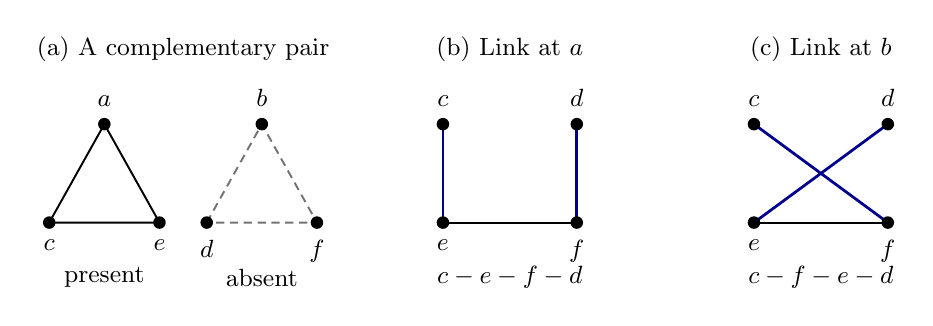
\begin{tikzpicture}[
  x=1cm,y=1cm,font=\small,
  vertex/.style={circle,fill=black,inner sep=1.6pt},
  every path/.style={line width=.7pt},
  matching/.style={draw=blue!55!black,line width=1pt}
]
\node at (1.7,2.2) {(a) A complementary pair};
\node at (5.85,2.2) {(b) Link at $a$};
\node at (9.8,2.2) {(c) Link at $b$};
\draw (0,0)--(.7,1.25)--(1.4,0)--cycle;
\node[vertex,label=above:$a$] at (.7,1.25) {};
\node[vertex,label=below:$c$] at (0,0) {};
\node[vertex,label=below:$e$] at (1.4,0) {};
\draw[densely dashed,draw=black!55] (2,0)--(2.7,1.25)--(3.4,0)--cycle;
\node[vertex,label=above:$b$] at (2.7,1.25) {};
\node[vertex,label=below:$d$] at (2,0) {};
\node[vertex,label=below:$f$] at (3.4,0) {};
\node at (.7,-.7) {present};
\node at (2.7,-.7) {absent};
\draw (5,0)--(6.7,0);
\draw[matching] (5,1.25)--(5,0) (6.7,0)--(6.7,1.25);
\node[vertex,label=above:$c$] at (5,1.25) {};
\node[vertex,label=above:$d$] at (6.7,1.25) {};
\node[vertex,label=below:$e$] at (5,0) {};
\node[vertex,label=below:$f$] at (6.7,0) {};
\node at (5.85,-.7) {$c-e-f-d$};
\draw (8.95,0)--(10.65,0);
\draw[matching] (8.95,1.25)--(10.65,0) (8.95,0)--(10.65,1.25);
\node[vertex,label=above:$c$] at (8.95,1.25) {};
\node[vertex,label=above:$d$] at (10.65,1.25) {};
\node[vertex,label=below:$e$] at (8.95,0) {};
\node[vertex,label=below:$f$] at (10.65,0) {};
\node at (9.8,-.7) {$c-f-e-d$};
\end{tikzpicture}
\caption{The complementary-triple rule forces opposite matchings.
Suppose the two triangles through $\{a,b\}$ are $\{a,b,c\}$ and
$\{a,b,d\}$. The links at $a$ and $b$, restricted to
$\{c,d,e,f\}$, share the edge $\{e,f\}$ and use opposite matchings
between $\{c,d\}$ and $\{e,f\}$ (shown in blue).
One of the two possible choices is drawn. The crossing in (c) is not a
vertex. Panel (a) shows one complementary pair for this choice.}
\label{fig:six-label-paths}
\end{figure}


\section{The obstruction on ten labels}\label{sec:ten-labels}

We prove that an admissible map $\mathbb{RP}^3\to\Delta^9$ cannot exist.
Its support complex would have tetrahedral facets. Each facet forces a
six-label triangle system on its complement; transporting these systems
between adjacent facets will constrain the whole complex.

\begin{lemma}\label{lem:facet-complement}
Suppose $f:\mathbb{RP}^3\to\Delta^9$ is admissible, let $K$ be its support
complex, and let $S$ be a tetrahedron of $K$. The triangles of $K$
contained in the six-element set $C=[10]\setminus S$ form a six-label
triangle system. In particular, two tetrahedra of $K$ cannot be disjoint.
\end{lemma}

\begin{proof}
Theorem~\ref{thm:equality-complex} says that $K$ is pure of
dimension three. A witness line $x$ for the facet $S$ has support exactly
$S$. The restriction of $f$ to $\mathbb P(x^\perp)\cong\mathbb{RP}^2$
uses only labels in $C$. It uses all six: otherwise the lower bound in
Proposition~\ref{thm:label-bound}, applied in dimension three,
would be violated. By Lemma~\ref{lem:six-from-map}, this restriction
supplies a six-label triangle system contained among the triangles of
$K$ on $C$.

There are no additional triangles on $C$. Otherwise some complementary
triples $T,C\setminus T$ would both be triangles of $K$. Take witness
lines for $S,T,C\setminus T$. In $\mathbb R^4$ there is a line
perpendicular to all three; their supports together contain all ten
labels, leaving that line no admissible label.

If a tetrahedron $S'$ were disjoint from $S$, its four triples would all
be triangles on $C$. This contradicts
Lemma~\ref{lem:six-properties}(2).
\end{proof}

The rest of the proof is purely combinatorial. We retain the notation
$K$ and write $\mathcal T_C$ for the triangle system on a facet
complement $C$. By Theorem~\ref{thm:equality-complex}, each
triangle of $K$ lies in a positive even number of tetrahedra.

\begin{lemma}\label{lem:two-tetrahedra}
Every triangle of $K$ belongs to exactly two tetrahedra.
\end{lemma}

\begin{proof}
First observe that if two tetrahedra differ by exchanging labels $a,b$,
the same exchange carries their complementary triangle systems to one
another. Their complements share five labels, on which both systems are
the triangles of $K$. After the exchange these triangles remain fixed,
so the systems agree everywhere by
Lemma~\ref{lem:six-properties}(4).

Suppose three tetrahedra $T\cup\{a\}$, $T\cup\{b\}$,
$T\cup\{c\}$ contain the same triangle $T$. Put
$R=[10]\setminus(T\cup\{a,b,c\})$, which has four elements. Transporting
the complementary systems successively by
\[
 R\cup\{b,c\}
 \xrightarrow{(a\ b)}R\cup\{a,c\}
 \xrightarrow{(b\ c)}R\cup\{a,b\}
 \xrightarrow{(c\ a)}R\cup\{b,c\}
\]
preserves the initial system. The composite fixes $R$ and exchanges $b$
and $c$, contradicting Lemma~\ref{lem:six-properties}(3). Thus at most
two tetrahedra contain any triangle. Positive even multiplicity gives
exactly two.
\end{proof}

For an edge $D$ of $K$, define its \emph{link graph} to have as vertices
the labels $v\notin D$ for which $D\cup\{v\}$ is a triangle, and as
edges the pairs $\{v,w\}$ for which $D\cup\{v,w\}$ is a tetrahedron.

\begin{lemma}\label{lem:short-links}
Every connected component of an edge link is a cycle of length three
or four.
\end{lemma}

\begin{proof}
Every vertex of an edge link has degree two by
Lemma~\ref{lem:two-tetrahedra}, so each component is a simple cycle.
We show that the link contains no path on five distinct vertices.

Suppose such a path has consecutive vertices $v_0,v_1,v_2,v_3,v_4$.
Let $R$ be the three labels outside $D\cup\{v_0,v_1,v_2,v_3,v_4\}$.
The four successive edges give tetrahedra
$D\cup\{v_i,v_{i+1}\}$, whose complementary systems are transported by
\[
\begin{aligned}
 R\cup\{v_2,v_3,v_4\}
 &\xrightarrow{(v_0\ v_2)} R\cup\{v_0,v_3,v_4\}
 \xrightarrow{(v_1\ v_3)} R\cup\{v_0,v_1,v_4\}\\
 &\xrightarrow{(v_2\ v_4)} R\cup\{v_0,v_1,v_2\}.
\end{aligned}
\]
The composite fixes $R$ and sends $v_4$ to $v_2$. Hence for every pair
$\{r,s\}\subset R$, the first system contains $\{v_4,r,s\}$ if and
only if the last contains $\{v_2,r,s\}$. The latter triple belongs to
both complementary sets, so its membership in either system is simply
its membership in $K$. The first system therefore has identical link
graphs at $v_4$ and $v_2$ when restricted to $R$. This contradicts
Lemma~\ref{lem:six-properties}(3). Every cycle of length at least five
contains such a path, proving the assertion.
\end{proof}

The short links let us describe every facet obtained by repeatedly
crossing a triangular face of one fixed tetrahedron. The description
will produce enough facets to contradict the complementary triangle
system.

\begin{lemma}\label{lem:partner-blocks}
Fix a tetrahedron $S$ of $K$. For $v\in S$, let $p(v)$ be the unique
label outside $S$ such that
$(S\setminus\{v\})\cup\{p(v)\}$ is a tetrahedron. For each distinct
value $y$ of $p$, set
\[
 B_y=p^{-1}(y)\cup\{y\}.
\]
The sets $B_y$ are disjoint and have at least two elements. For every
choice $q_y\in B_y$, the set
\[
 \bigcup_{y\in p(S)}(B_y\setminus\{q_y\})
\]
is a tetrahedron. Moreover, every tetrahedron of $K$ contains at least two
elements of one of these blocks.
\end{lemma}

\begin{proof}
The partner $p(v)$ exists and is unique by
Lemma~\ref{lem:two-tetrahedra}, applied to $S\setminus\{v\}$. It lies
outside $S$, since the only tetrahedron on the vertices of $S$ is $S$
itself. The stated disjointness and lower size bound are immediate.

We first prove that replacing $v$ by $a=p(v)$ leaves the collection of
blocks unchanged. Put $S'=(S\setminus\{v\})\cup\{a\}$ and let $p'$
be its partner map. We have $p'(a)=v$. For $w\in S\setminus\{v\}$,
put $D=S\setminus\{v,w\}$ and $b=p(w)$. The link of $D$ contains
the edges
\[
 \{v,w\},\qquad \{w,a\},\qquad \{v,b\}.
\]
If $a=b$, these form a three-cycle. Since every link vertex has degree
two, that cycle is a whole component, and the other tetrahedron on
$D\cup\{a\}$ is $D\cup\{a,v\}$. Thus $p'(w)=v$.
If $a\ne b$, the displayed edges form the path $a,w,v,b$ on four
distinct vertices. Lemma~\ref{lem:short-links} forces it to complete
to a four-cycle, with the edge $\{a,b\}$. Thus $p'(w)=b=p(w)$.
The two cases are illustrated in Figure~\ref{fig:partner-links}.
We have proved
\[
 p'(a)=v,\qquad
 p'(w)=
 \begin{cases}
 v,&p(w)=a,\\
 p(w),&p(w)\ne a.
 \end{cases}
\]
\begin{figure}[tbp]
\centering
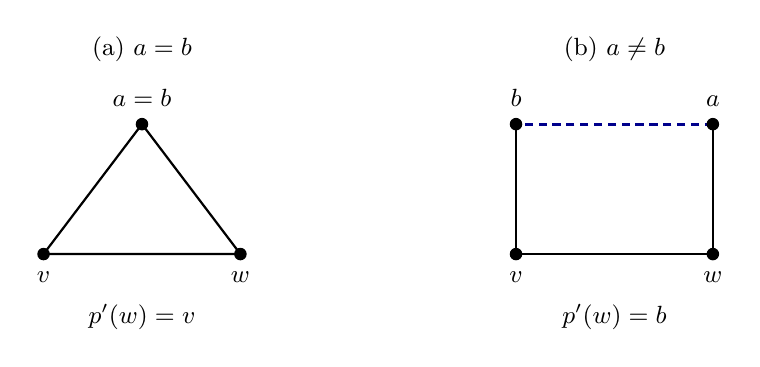
\begin{tikzpicture}[
  x=1cm,y=1cm,font=\small,
  vertex/.style={circle,fill=black,inner sep=1.6pt},
  every path/.style={line width=.8pt}
]
\node at (1.25,2.6) {(a) $a=b$};
\node at (7.25,2.6) {(b) $a\ne b$};
\draw (0,0)--(2.5,0)--(1.25,1.65)--cycle;
\node[vertex,label=below:$v$] at (0,0) {};
\node[vertex,label=below:$w$] at (2.5,0) {};
\node[vertex,label=above:{$a=b$}] at (1.25,1.65) {};
\node at (1.25,-.8) {$p'(w)=v$};
\draw (6,1.65)--(6,0)--(8.5,0)--(8.5,1.65);
\draw[blue!55!black,densely dashed,line width=1pt] (8.5,1.65)--(6,1.65);
\node[vertex,label=below:$v$] at (6,0) {};
\node[vertex,label=below:$w$] at (8.5,0) {};
\node[vertex,label=above:$b$] at (6,1.65) {};
\node[vertex,label=above:$a$] at (8.5,1.65) {};
\node at (7.25,-.8) {$p'(w)=b$};
\end{tikzpicture}
\caption{The two partner updates in the link of
$D=S\setminus\{v,w\}$. Put $a=p(v)$ and $b=p(w)$, and replace
$v$ by $a$ in the tetrahedron $S$. The new partner map is $p'$.
The known edges $\{v,w\}$, $\{w,a\}$ and $\{v,b\}$ form a triangle
when $a=b$. When $a\ne b$, they form a path on four vertices; the
short-link condition forces the closing edge $\{a,b\}$ (dashed).
In both cases $p'(a)=v$, and the blocks retain their elements.}
\label{fig:partner-links}
\end{figure}


The block formerly indexed by $a$ is now indexed by $v$ and has the
same elements; all other blocks are unchanged.

The tetrahedron $S$ contains all elements of each block except its
indexing partner. The same is true after any such exchange, by block
invariance. To change the omitted element of a block from $q$ to $u$,
replace the present element $u$ by its partner $q$. Doing this once
in each block where a change is wanted realizes every possible choice
of omissions. These sets have cardinality four, since
$\sum_y(|B_y|-1)=|S|=4$.

Finally, suppose a tetrahedron $T$ met each block in at most one
element. In each block omit that element if present, and otherwise
omit any element. The resulting tetrahedron lies in the union of the
blocks and is disjoint from $T$, contrary to
Lemma~\ref{lem:facet-complement}.
\end{proof}

\begin{theorem}\label{thm:no-ten-labels}
There is no admissible map $\mathbb{RP}^3\to\Delta^9$.
\end{theorem}

\begin{proof}
Assume such a map exists and fix a tetrahedron $S$ of its support
complex. Let $t$ be the number of blocks in
Lemma~\ref{lem:partner-blocks}, and let $R$ be the set of labels outside
their union. The blocks contain $4+t$ labels in total, so
\[
 1\le t\le4,\qquad |R|=6-t.
\]
If $t=4$, each block has size two and $S$ meets each in just one
element, contradicting the last assertion of
Lemma~\ref{lem:partner-blocks}. Thus $t\le3$.

There is no triangle entirely in $R$. By purity, such a triangle would
extend to a tetrahedron; its one remaining vertex could not supply two
vertices in a block. On the other hand, $R$ is contained in
$[10]\setminus S$, where every four labels contain a triangle by
Lemmas~\ref{lem:facet-complement} and~\ref{lem:six-properties}(2).
Consequently $|R|\le3$, and therefore $t\ge3$.

It follows that $t=3$, $|R|=3$, and the block sizes are $3,2,2$,
as in Figure~\ref{fig:partner-blocks}.
\begin{figure}[tbp]
\centering
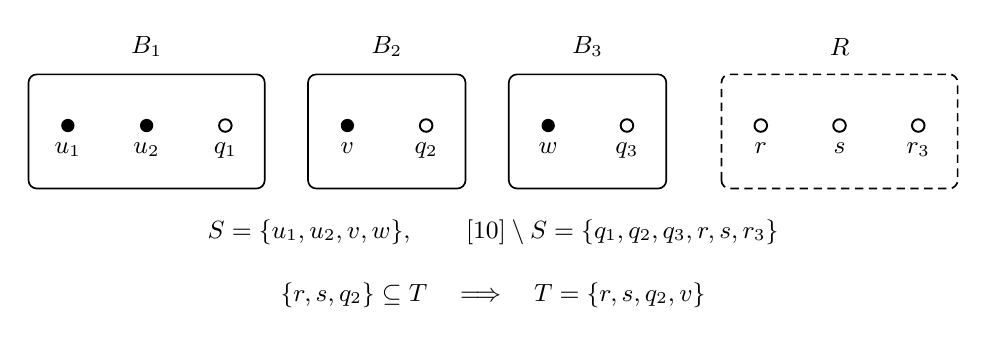
\begin{tikzpicture}[
  x=1cm,y=1cm,font=\small,
  present/.style={circle,fill=black,inner sep=1.7pt},
  omitted/.style={circle,draw=black,fill=white,inner sep=1.6pt,line width=.7pt},
  every path/.style={line width=.6pt}
]
\draw[rounded corners=3pt] (0,.35) rectangle (3,1.8);
\draw[rounded corners=3pt] (3.55,.35) rectangle (5.55,1.8);
\draw[rounded corners=3pt] (6.1,.35) rectangle (8.1,1.8);
\draw[rounded corners=3pt,densely dashed] (8.8,.35) rectangle (11.8,1.8);
\node at (1.5,2.15) {$B_1$};
\node at (4.55,2.15) {$B_2$};
\node at (7.1,2.15) {$B_3$};
\node at (10.3,2.15) {$R$};
\node[present,label=below:$u_1$] at (.5,1.15) {};
\node[present,label=below:$u_2$] at (1.5,1.15) {};
\node[omitted,label=below:$q_1$] at (2.5,1.15) {};
\node[present,label=below:$v$] at (4.05,1.15) {};
\node[omitted,label=below:$q_2$] at (5.05,1.15) {};
\node[present,label=below:$w$] at (6.6,1.15) {};
\node[omitted,label=below:$q_3$] at (7.6,1.15) {};
\node[omitted,label=below:$r$] at (9.3,1.15) {};
\node[omitted,label=below:$s$] at (10.3,1.15) {};
\node[omitted,label=below:$r_3$] at (11.3,1.15) {};
\node at (5.9,-.2) {$S=\{u_1,u_2,v,w\},\qquad [10]\setminus S=\{q_1,q_2,q_3,r,s,r_3\}$};
\node at (5.9,-1) {$\{r,s,q_2\}\subseteq T\quad\Longrightarrow\quad T=\{r,s,q_2,v\}$};
\end{tikzpicture}
\caption{The only remaining block sizes are $3,2,2$, with three
labels in $R$ outside the blocks. Filled dots are the vertices of the
fixed tetrahedron $S$; the omitted block elements are $q_1,q_2,q_3$.
Every tetrahedron must contain two vertices of one block. After
relabeling the two-element blocks, the final argument selects a triangle
$\{r,s,q_2\}$ with $r,s\in R$. Its only possible tetrahedral extension
is obtained by adjoining $v$, contradicting the two required extensions.}
\label{fig:partner-blocks}
\end{figure}


The complement of $S$ consists of $R$ and one omitted element from
each block. Choose two distinct labels $r,s\in R$. In the triangle
system on this complement, $\{r,s\}$ belongs to two distinct triangles.
Their third vertices cannot be in $R$, because $R$ contains no
triangle. They are therefore two distinct omitted block elements.
Only one block has size three, so at least one of these triangles is
$\{r,s,z\}$ with $z$ in a block $B$ of size two.

Every tetrahedron containing $\{r,s,z\}$ must contain two vertices of
some block. As $r,s$ lie outside all blocks, its fourth vertex must be
the other element of $B$. Thus this triangle belongs to at most one
tetrahedron, contradicting Lemma~\ref{lem:two-tetrahedra}.
\end{proof}

\section{The diameter obstruction}
\label{sec:conclusion}

All ingredients now apply to the projector set in Theorem~\ref{thm:main}.

\begin{proof}[Proof of Theorem~\ref{thm:main}]
Lemma~\ref{lem:projector-geometry}, with $k=4$, proves compactness and
identifies the trace-one affine space with Euclidean $\mathbb R^9$.
It also gives the exact diameter $\sqrt2$. If ten subsets of strictly
smaller diameter covered $X$, Lemma~\ref{lem:cover-to-map} would supply
an admissible map $\mathbb{RP}^3\to\Delta^9$. This contradicts
Theorem~\ref{thm:no-ten-labels}.
\end{proof}

The spherical geometry of this witness also gives counterexamples in
all higher dimensions. We use the familiar construction of adjoining
points at diameter distance; see
\cite[Lemma~9]{HinrichsRichter2003} and
\cite[proof of Corollary~1]{Bondarenko2014}. The following Gram-matrix
description adds all the new points at once.

\begin{corollary}\label{cor:higher-dimensions}
For every integer $d\geq9$, there is a compact subset of $\mathbb R^d$
of diameter $\sqrt2$ that cannot be covered by $d+1$ subsets of
strictly smaller diameter.
\end{corollary}

\begin{proof}
The case $d=9$ is Theorem~\ref{thm:main}. For $d=9+s$ with $s\geq1$,
translate its projector set to
\[
 Y=\{P_x-\tfrac14 I:x\in\mathbb{RP}^3\}
\]
in the nine-dimensional space of trace-zero symmetric matrices.
Every $y\in Y$ has $\|y\|_F^2=3/4$. In an orthogonal copy of
$\mathbb R^s$, choose vectors $v_1,\ldots,v_s$ with Gram matrix
\[
 (\langle v_i,v_j\rangle)_{i,j=1}^s
 =I_s+\tfrac14\mathbf1\mathbf1^{\mathsf T},
 \qquad \mathbf1=(1,\ldots,1)^{\mathsf T}.
\]
Such vectors exist because the displayed matrix is positive definite.
They satisfy $\|v_i\|^2=5/4$ and
$\|v_i-v_j\|^2=2$ for $i\ne j$. Therefore the compact set
\[
 Z=(Y\times\{0\})\cup\{(0,v_i):1\leq i\leq s\}
 \subset\mathbb R^9\oplus\mathbb R^s
\]
has diameter $\sqrt2$: each new point is at that distance from every
point of $Y\times\{0\}$ and from every other new point.

A subset of $Z$ of strictly smaller diameter containing a new point
can contain neither a second new point nor a point of $Y\times\{0\}$.
Thus a cover of $Z$ by at most $d+1=10+s$ such subsets would leave
at most ten subsets to cover $Y\times\{0\}$. This contradicts
Theorem~\ref{thm:main}, since translation preserves diameter and the
number of covering sets.
\end{proof}

\bibliographystyle{plain}
\bibliography{references}
\end{document}
